
% https://services.math.duke.edu/~ng/knotgallery.html

We will start by computing the \Ainf algebra associated with the Legendrian
projection of some very simple knots shown in figure \ref{fig:simple_knots}. 

\begin{figure}
\centering
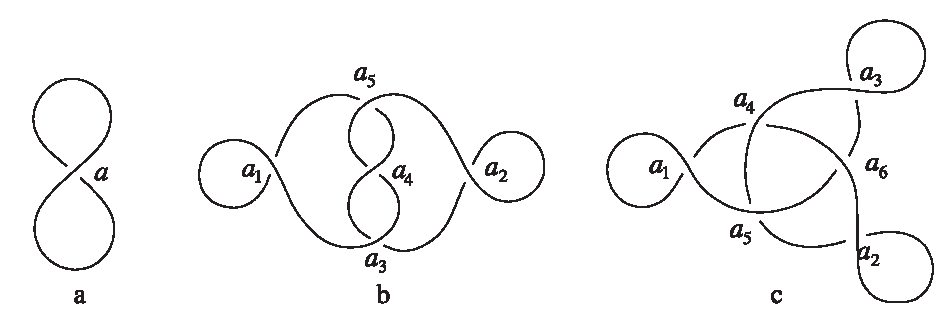
\includegraphics[width=.8\textwidth]{figs/simple_knots.pdf}
\caption{$k$ sided polygon.}
\label{fig:simple_knots}
\end{figure}

\begin{exmp} Let $Y_0$ be the Lagrangian projection of the Legendrian unknot
$L_0$, shown figure (\ref{fig:simple_knots}a). The winding number $\sigma(L_0) =
0$, so the grading takes values in $\Gamma = \Z$. There is only one crossing
$a$, with degree $|a| = 1$. So $A = \Z_2\<{a}$. The set of immersions
$\tilde{W}_k(Y_0)$ is empty for $k > 1$ and $\tilde{W}_k(Y_0) = \{ f_1, f_2 \}$,
where $f_1$ and $f_2$ are the immersions whose image are the two bounded
components of $\R^2 \setminus Y_a$. Considering the sign of the quadrants of the
crossing, we observe that both $f_1$ and $f_2$ are admissible. Hence $m_k = 0$
for all $k>0$ and $m_0(1) = \#_2\{f_1,f_2\} a = 0$.
\end{exmp}

\begin{exmp}
Consider $Y_r$ given by figure (\ref{fig:simple_knots}b), the Lagrangian
projection of the Legendrian Right-handed trefoil knot $L_r$. The winding number
$r=0$ again, so $\Gamma = \Z$. There is $5$ crossings, $A = \<{b_1, b_2, b_3,
a_1, a_2}$, and the grading is given by
\[ |a_i| = 1, \quad |b_i| = 0. \]
There is two admissible immersions with one vertex, there is also four with two
vertices and two with four (see figure \ref{fig:simple_knots}b). So $m$ is given
by

\begin{align*}
m_0(1) = m_1(b_1) = m_1(b_3) &= a_1 + a_2 \\
m_3(b_1,b_2,b_3) &= a_1 \\
m_3(b_3,b_2,b_1) &= a_2.
\end{align*}
And all other terms are zero.

\end{exmp}


We will also have a look at two other slightly more complicated knots, shown in
figure \ref{fig:chek_elias_knots}. Later we will see that with the invariant
induced by the associated \Ainf algebra one are able to distinguish this two
knots, even though both knots has the same classical invariants.

\begin{figure}
\centering
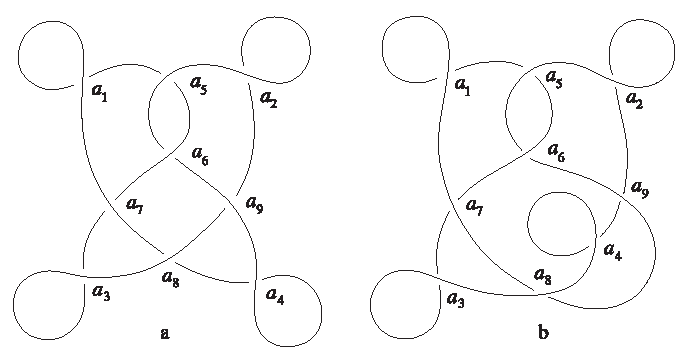
\includegraphics[width=.8\textwidth]{figs/chek_elias_knots.pdf}
\caption{$k$ sided polygon.}
\label{fig:chek_elias_knots}
\end{figure}

\begin{exmp}
Let $Y_a$ and $Y_b$ be given by figure (\ref{fig:chek_elias_knots}). 
For both of the knots the winding number $r=0$ and there is $9$ crossings,
enumerated as shown in the figure. Let's first consider diagram (a), the grading
is given by
\[ |a_i| = 1, \quad |a_5| = 2, \quad |a_6| = -2 \q\tand |a_j| = 0, \]
where $i = 1,...,4$ and $j = 7,...,9$. The \Ainf maps $m_i$ is given by

\begin{align*}
m_0(1) &= a_1 + a_2 + a_3 + a_4, \\
m_3(a_7,a_6,a_5) = m_1(a_7) &= a_1, \\
m_3(a_5,a_6,a_9) = m_1(a_2) &= a_2, \\
m_2(a_8,a_7) &= a_3, \\
m_2(a_9,a_8) &= a_4.
\end{align*}
And all other terms are zero. Now les's consider the second diagram. The grading
is given by
\[ |b_i| = 1 \q\tand |b_j| = 0, \]
where $i = 1,...,4$ and $j = 5,...,9$. The \Ainf maps are given by

\begin{align*}
m_0(1) &= b_1 + b_2 + b_3 + b_4, \\
m_3(b_7,b_6,b_5) = m_1(b_7) &= b_1, \\
m_3(b_9,b_8,b_5) = m_1(b_5) &= b_1, \\
m_3(b_5,b_6,b_9) = m_1(b_9) &= b_2, \\
m_2(b_8,b_7) &= b_3, \\
m_2(b_9,b_8) &= b_4.
\end{align*}
And all other terms are zero. So clearly this are different \Ainf algebras, but
that is not in itself a sufficent argument for to say that they are different
knots.

\end{exmp}
